%------------------------------------------------------------
% Description : Line integrals, diff forms
% Author      : taxus-d <iliya.t@mail.ru>
% Created at  : Sun Nov 13 16:01:51 MSK 2016
%------------------------------------------------------------
\documentclass[12pt,timbord]{../../../notes}
\usepackage{silence}
\WarningFilter{latex}{Reference}
\graphicspath{{../../img/}}

\begin{document}
\paragraph{\underdev Интеграл от дифференциальной формы по пути}
\label{par:lineint::defs}
Параграфы со значком  <<\underdev>> лучше не читать, они недопилены.

\subparagraph{Дифференциальные формы.} 
Начать лучше с полилинейных форм.
\begin{defn}\label{defn:lineint::defs::linform}
  Пусть $L$~--- линейное пространство над полем $K$. Тогда функция $A\colon L^k\to K$, линейная по
  каждому из своих аргументов, называется $k$-линейной формой.
\end{defn}

\note{<ну его>}\note{<потом лучше напишу>}

Нам тут хватит и 1-форм, так что
\begin{defn}\label{defn:lineint::defs::diffform}
  Дифференциальной 1-формой можно назвать отображение из $\R^n$ в линейную (по $h$) форму, $P\in C^0$
  \[
    \omega = \langle P(x), \del x(x,h)\rangle
  \]
  Но это как-то не очень ({а что такое дифференциал?}).
\end{defn}

\subparagraph{Гладкие пути.}

\begin{defn}\label{defn:lineint::defs::smoothpath}
  Пусть $\gamma\colon [a;b]\subset \R \to \R^n$. Тогда $\gamma$ называется путём в пространстве
  $\R^n$.
  \begin{itemize}
    \item Путь гладкий, если $\gamma\in C^1$,
    \item путь регулярный, если $\rk\gamma' \geqslant 1$,
    \item путь простой, если $\gamma$~--- биекция.
  \end{itemize}
\end{defn}

\begin{defn}\label{defn:lineint::defs::curve}
  Образ $\Gamma = \gamma([a;b]) \subset \R^n$ называется \emph{кривой} в $\R^n$. Ещё говорят, что
  $\Gamma$~--- носитель пути $\gamma$, а $\gamma$~--- параметризация $\Gamma$.
\end{defn}

\begin{rem*}
  Путь простой $\Leftrightarrow$ кривая не имеет самопересечений.
\end{rem*}

\begin{defn}\label{defn:lineint::defs::pathorient}
  Будем говорить, что простые пути имеют одинаковую ориентацию, если
  \[
    \gamma_1(a_1)=\gamma_2(a_2)\; \gamma_1(b_1) = \gamma_2(b_2)
  \]
  и противоположную, если всё наоборот.
  Тут ещё введу нестандартное обозначение, но так жить проще $\ddot\smile$.
  \begin{itemize}
    \item $\coori$~--- одинаковая ориентация
    \item $\conori$~--- противоположная ориентация
  \end{itemize}
\end{defn}
\begin{rem*}
  Для биективных параметризаций видимо просто нет другого выбора. С петлями всё будет интереснее.
\end{rem*}

\subparagraph{Интегралы от форм по пути}

\begin{defn}\label{defn:lineint::defs::lineint}
  Просто возьмём и определим интегралы по простому гладкому пути от 1-форм так:
  \[
    I = \int_\gamma \omega := \int_a^b \langle P,\dot x(t)\rangle \del t
  \]
\end{defn}

\begin{prop}[Корректность определения выше]\label{prop:lineint::defs::lineint}
  Интеграл по пути не зависит от параметризации.
\end{prop}
\begin{ittproof}
  Пусть $\gamma_1, \gamma_2$~--- параметризации $\Gamma$, одинаково ориентированы. Докажем,что
  \[
    I_1 = \int_{\gamma_1} \omega = \int_{\gamma_2} \omega = I_2 
  \]
  Поскольку $\gamma_1, \gamma_2$~--- биекции, $\exists\, \varphi \colon $
  $t_2 = \varphi(t_1)$, тоже биекция, такого сорта:
   $t_1\xmapsto{\gamma_1}x\xmapsto{\gamma_2^{-1}}t_2$
  Тогда 
  \[
    I_2  = \int_{a_2}^{b_2} \langle P(\gamma_2(t_2)), \partial_{t_2}\gamma_2(t_2)\rangle \,\del t_2 = 
    \int_{a_1}^{b_1} \langle P(\underbrace{\gamma_2(\varphi(t_1))}_x), 
  \partial_{t_2}\gamma_2(t_2))\rangle \, \partial_{t_1}\varphi(t_1) \,\del t_1
  \]
  Покажем, что $\partial_{t_2}\gamma_2(t_2) \partial_{t_1}\varphi = \partial_{t_1}
  \gamma_1(t_1)$. Это просто следует равенства $\gamma_1(t_1)=\gamma_2(t_2)$, если его
  продифференцировать по $t_1$. Так что
  \[
    \int_{a_1}^{b_1} \langle P(x), 
  \partial_{t_1}\gamma_1(t_1))\rangle \, \bigl(\partial_{t_1}\varphi(t_1) \bigr)^{-1}
  \partial_{t_1}\varphi(t_1) \,\del t_1   = I_1
  \]
\end{ittproof}
\begin{rem}
  Если $\gamma_1 \conori \gamma_2$, то $I_2 = - I_1$.
\end{rem}
\begin{rem}
  Если рассматривать только одинаково ориентированые пути, то
  \[
    \int_{\gamma} \omega = \int_{\Gamma} \omega
  \]
\end{rem}

\begin{rem}
  Если $\Gamma$ разбивается на непересекащиеся $\Gamma_1$, $\Gamma_2$, то 
  \[
    \int_\Gamma \omega = \int_{\Gamma_1} \omega + \int_{\Gamma_2} \omega
  \]
\end{rem}

\subparagraph{Петли и интегралы по ним}


\begin{defn}\label{defn:lineint::defs::loop}
  Кривая $\Gamma$~--- петля, если для всякой её параметризации $\gamma(a) = \gamma(b)$. 
  Петля называется простой, если $\exists\, \colon \gamma\vert_{[a;b)}$~--- биекция.
\end{defn}
\begin{rem*}
  Плохие петли можно разбивать на простые.
\end{rem*}

\begin{defn}\label{defn:lineint::defs::loopint}
  Пусть $\Gamma$~--- простая петля. Тогда 
  \[
    I = \oint_\gamma \omega := \int_a^b \langle P,\dot x(t)\rangle \del t
  \]
\end{defn}
\begin{prop}\label{prop:lineint::defs::loopint}
  Определение выше корректно, и не зависит от выбора <<начала>> петли. 
\end{prop}  
\begin{itlproof}
  Можно рассмотреть 2 разные параметризации и разбить на 2 куска. Дальше работает определение
  интеграла по простому пути.
\end{itlproof}

\begin{rem*}
  Чтобы посчитать интегралы по всем остальным путям, их нужно разбивать на прострые пути и
  простые петли
\end{rem*}


\paragraph{Точные формы}
\label{par:lineint::precforms}

\begin{defn}\label{defn:lineint::precforms::def}
  1-форма $\omega$ называется точной в $G$, если $\exists\, \Phi\colon G\subset \R^n\to \R$, такая что
  $\omega =  \del \Phi$. $\Phi$ в таком случае называется потенциалом, а сама форма ещё иногда
  назыается потенциальной.
\end{defn}
\begin{exmp*}
  Работа в физике.
\end{exmp*}

\begin{thrm}\label{thrm:lineint::precforms::precint}
  Пусть $\omega$~--- точная форма в  $G$, $\Gamma \subset G$, $\gamma(a)=A$, $\gamma(b)=B$
  Тогда
  \[
    \int_\gamma \omega = \Phi(B) - \Phi(A)
  \]
\end{thrm}
\begin{ittproof}
  $\langle P, x \rangle = (\Phi \circ \gamma)' (t)$. Дальше уже тривиально из непрерывности
  $\Phi$.
\end{ittproof}

\begin{thrm}\label{thrm:lineint::precforms::precint2}
  Пусть $\omega$~--- точная форма в  $G$, $\Gamma_1, \Gamma_2 \subset G$,
  $\gamma_{1,2}(a)=A$, $\gamma_{1|2}(b)=B$.
  Тогда
  \[
    \int_\gamma \omega = \Phi(B) - \Phi(A)
  \]
\end{thrm}

\begin{thrm}\label{thrm:lineint::precforms::loopint}
  Пусть $\omega$~--- точная форма в  $G$, $\Gamma \subset G$~--- петля
  Тогда
  \[
    \oint_\gamma \omega = 0
  \]
\end{thrm}

\begin{thrm}\label{thrm:lineint::precforms::critprec}
  Пусть $\omega$~--- форма в  $G$, и $\int_\gamma \omega $ не зависит от пути при фиксировнных
  концах. Тогда $\omega$~--- точна.
\end{thrm}

\begin{ittproof}
  Надо показать, что $\partial_i \Phi = P^i$. В этом месте можно забить на общности и объявить
  $n=2$. Докажем, что $\partial_x \Phi = P^1$. Поскольку от пути ничего не зависит,
  \[
    \pder{\Phi}{x}(x,y) = \lim_{\Delta x\to 0}\frac{\Phi(x+\Delta x)- \Phi(x,y)}{\Delta x} = 
    \lim_{\Delta x\to 0} \frac{1}{\Delta x} \left(\int_A^{{(x+\Delta x,y)}} \omega - 
    \int_A^{(x,y)} \omega\right)
  \]
  А это по сути интеграл по пути, соединяющем $(x+\Delta x, y)$ и $(x, y)$. А здесь уже можно
  взять приличную кривую (прямую) с правильной параметризацией, и воспользоваться теоремой о
  среднем.
  \[
    \cdots = \lim_{\Delta x \to 0} \frac{1}{\Delta x} \int_{x}^{x+\Delta x} P(t, y) \del t = 
    \lim_{\Delta x \to 0} P(\xi, y) = P(x,y)
  \]
  Последнее равенство верно по непрерывности.
\end{ittproof}

\begin{thrm}\label{thrm:lineint::precforms::critprecloop}
  $\displaystyle \oint \omega =0 \Rightarrow \omega$~--- точна
\end{thrm}

\begin{thrm}\label{thrm:lineint::precforms::precrecloop}
  Пусть $G$, $\oint \omega =0 $ для любой прямоугольной петли. Тогда $\omega$~--- точна.
\end{thrm}
\begin{ittproof}
  Аккуратно свести к теореме~\ref{thrm:lineint::precforms::critprec}, там всё будет работать и с
  путями, параллельными осям координат.
\end{ittproof}

\paragraph{Замкнутые формы}
\label{par:lineint::closforms}
Здесь уже окончательно забиваем на все $n \geqslant 2$. Там, в целом, понятно как обобщать.
Тут всюду $\omega =  P(x,y) \del x + Q(x,y) \del y$
\begin{defn}\label{defn:lineint::closforms::closform}
  Форма $\omega$ замкнута в $G$, если
  \[
    \forall\, A \in G \; \exists U (A) \colon \exists\, \Phi_U\colon U\to R \;\:\: \omega = \del
    \Phi_U
  \]
  короче, локально точна.
\end{defn}

\begin{thrm}\label{thrm:lineint::closforms::nessdiff}
  Пусть $\omega$~--- гладкая форма в $G$. Тогда если $\omega$ замкнута,
  $\partial_y P = \partial_x Q$ в $G$.
\end{thrm}
\begin{ittproof}
  Очевидно следует из <<локальной точности>>.
\end{ittproof}

\begin{thrm}\label{thrm:lineint::closforms::suffdiff}
  Пусть $\omega$~--- гладкая форма в $G$. Тогда если $\partial_y P = \partial_x Q$ в $G$, то
  $\omega$ замкнута.  
\end{thrm}
\begin{ittproof}
  Выберем произвольную $A$, тогда $U_\varepsilon(A) \subset G$. Надо попробовать построить
  потенциал. Например так $\Phi(B) = \int_{\gamma_1 + \gamma_2} \omega$. 
  Докажем, что $\partial_x \Phi = P$, $\partial_y \Phi = Q$.

  \begin{minipage}{0.48\linewidth}
    \begin{tikzpicture}[scale=2]
      \coordinate[label=$A$] (A) at (0,0);
      \coordinate[label=$B$] (B) at (0.7,1);
      \coordinate[label=$C$] (C) at (1.1,1);
      \coordinate (D) at (0.7,0);
      \coordinate (E) at (1.1,0);
      \draw (0,0) circle (2);
      \begin{scope}[decoration={
            markings,
          mark=at position 0.5 with {\arrow{>}}}
        ] 
        \draw[postaction={decorate}] (A)-- node[below]{$\gamma_1$} (D);
        \draw[postaction={decorate}] (D)-- node[left]{$\gamma_2$}(B);
        \draw[postaction={decorate}] (D)-- node[below]{$\gamma_3$}(E);
        \draw[postaction={decorate}] (E)-- node[right]{$\gamma_4$}(C);
      \end{scope}
    \end{tikzpicture}
  \end{minipage}\hfill
  \begin{minipage}{0.48\linewidth}
    \[
      \begin{split}
        \Delta \Phi &= \Phi(C)-\Phi(B) = \int_{\gamma_4} \omega - \int_{\gamma_2} \omega +
        \int_{\gamma_3} \omega \\
        &= \int_{y_A}^y Q(x+\Delta x, t) \del t 
        - \int_{y_A}^y Q(x, t) \del t + \int_{x}^{x+\Delta x} P(t, y_A) \del t
      \end{split}
    \]
    Последний сходится к $P(x,y_0)\del x$, а первые два надо немного преобразовать
    \[
      \frac{1}{\Delta x} \left(\int_{\gamma_4} \omega 0 \int_{\gamma_2} \omega \right)
      = \int_{y_0}^y \left(\frac{Q(x+\Delta x,t ) - Q(x,t)}{\Delta x}\right) \del t
    \]
    Подинтегральную функцию можно представить как последовательность $f_n \rightrightarrows Q'$.
    \[
      \left| \frac{Q(x+\lfrac 1 n )- Q(x)}{\frac 1 n} - Q'(x)\right| = |Q'(\xi) - Q(x) |
      <\varepsilon
    \]
    а функция $Q'$ равномерно непрерывна на $[x, x+ \Delta x]$, ибо он отрезок. Так что можно
    поменять местами предел и интеграл.
    \[
      \cdots = \int_{y_0}^y \pder{Q}{x}(x,y) \del t = \int_{y_0}^y \pder{P}{y} (x,y) = \Delta P
    \]
  \end{minipage}
    Если сложить с оставшимся куском, то как раз и выйдет $P$. С равенством $Q$ вроде все
    попроще, там нужно считать приращение всего лишь по одному пути.
\end{ittproof}
\begin{rem}
  Бывают замкнутые, но не точные формы. Например $\omega = \dfrac{-y \del x + x \del y}{x^2 +
  y^2}$. Она замкнута, а вот $\oint_\gamma w$ по окружности вокруг $0$ не 0.
\end{rem}

\paragraph{Первообразная замкнутой формы вдоль пути}
\label{par:lineint::closintpath}

Сначала можно отметить, что $\Gamma = \gamma\bigl([a;b]\bigr)$~--- компакт. Так что вроде можно
пользоваться теоремой о конечном подпокрытии.
\begin{lem}\label{thrm:lineint::closintpath::potdiff}
    Пусть $G$~--- область, $\omega$~--- гладкая точная форма в $G$, 
    а $\Phi, \Psi$~--- две её первообразные в $G$. Тогда $\Phi-\Psi\equiv C\in \R$.
\end{lem}

\begin{thrm}\label{thrm:lineint::closintpath}
  Пусть $\omega$ замкнута в $G$, $\Gamma=\gamma([a;b])$. Тогда существует первообразная вдоль пути
  $\gamma$ и  $\dint_\gamma \omega = f(b) - f(a)$.
\end{thrm}

\begin{ittproof}
  Поскольку кривая компактна, в любом её покрытии можно выделить конечное подпокрытие. Собственно,
  будем рассматривать покрытие открытыми кругами $U(p_i)$. Пусть $\Phi_i$~--- произвольная
  первообразная в $U_i$. Заменим $\Phi_i$ $\widetilde{\Phi_i}$, так что 
  $\widetilde{\Phi}_{i+1}= \widetilde{\Phi}_{i}$ на $U_{i+1} \cap U_i$, $\widetilde{U}_0=U_0$.

  Выберем параметризацию, тогда $p_i$  соответствуют $t_0=a< t_1 <\cdots < t_n = b$
  Теперь выберем $f(\gamma(t)) = \widetilde{\Phi}_k(\gamma(t))$, $\gamma(t) \in U_k$.
  Здесь вроде можно прожить и без простоты пути.\note{вообще первообразную вдоль пути нигде не
  определяли, так что можно считать конструкцию, построенную выше, определением}

  Теперь ещё выберем $q_i \in U_{i+1} \cap U_i$, $\{\gamma_j\} =$ пути от $ p_i$ до $q_i \cap$
  пути от $q_i$ до $p_{i+1}$. Тогда
  \[
    \in _\gamma \omega = \sum_j\int_{\gamma_j} =  \widetilde{\Phi}(p_n) - \widetilde{\Phi}{p_0} =
    f(b) - f(a)
  \]
\end{ittproof}

\paragraph{\underdev Гомотопия путей}
\label{par:lineint::homotopy}

\begin{defn}\label{defn:lineint::homotopy::set}
  Непрерывным семейством путей называется непрерывная функция $g\colon [0;1]\times[a;b]\to \R^n$.
  Часто обозначается так: $\gamma_s(t) = g(s,t)$. \note{По-хорошему там должны быть топологические
  пространства, но не сегодня и не сейчас .}
\end{defn}

\begin{defn}[$\ddot\sim$]\label{defn:lineint::homotopy::paths}
  Пусть $\gamma_1, \gamma_2\colon [a;b]\to G$, $\gamma_1(a)=
  \gamma_2(a)$,$\gamma_1(b)=\gamma_2(b)$. Тогда утверждается, что пути гомотопны, если существует
  семейство $\gamma_s(t)\colon$ $\gamma_{s_1} = \gamma_1$, $\gamma_{s_2} = \gamma_2$.
\end{defn}
\begin{rem*}
  Таки отношение эквивалентности.
\end{rem*}

\begin{thrm}\label{thrm:lineint::homotopy::lineinteq}
  Пусть $\omega$~--- замкнутая форма в области $G$, $\gamma_1 \sim \gamma_2$. Тогда
  \[
    \int _{\gamma_1} \omega = \int_{\gamma_2} \omega
  \]
\end{thrm} 
\begin{thrm}\label{thrm:lineint::homotopy::loopinteq}
  Пусть $\omega$~--- замкнутая форма в области $G$, $\gamma_1 \sim \gamma_2$~--- гомотопные петли.
  Тогда
  \[
    \oint _{\gamma_1} \omega = \oint_{\gamma_2} \omega
  \]
\end{thrm} 
\begin{rem*}
  Доказывать я это пока не буду, иначе это будет выглядеть как-то так:\par
  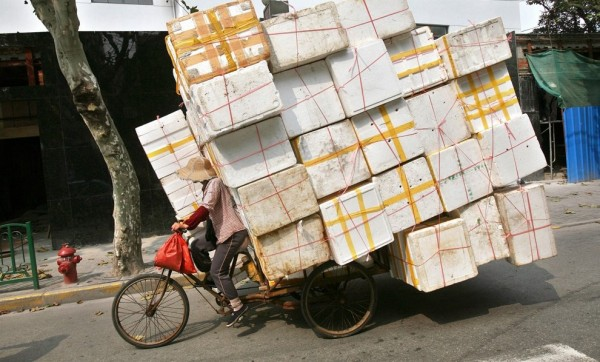
\includegraphics[width=0.7\linewidth]{overloaded}
\end{rem*}



\end{document}
% vim: wrapmargin=3
